\chapter{Simulation des robots}
\chaptermark{Robots}
\label{chapitre:robots}
	
	\section{Introduction}

		L'environnement dans lequel doivent évoluer les robots à été défini dans le \textsc{Chapitre}~\ref{chapitre:environnement}. Il est maintenant temps de simuler les \gls{ROV}s. Pour ce faire, nous allons devoir décrire les paramètres mécaniques des robots \argos{} et \atoll{}, et décrire le comportement de leurs capteurs et actionneurs à simuler. A la fin de cette partie nous devrions être en mesure de pleinement simuler les robots dans leur environnement et le simulateur complet devrait ainsi respecter toutes les exigences présentées dans le \textsc{Chapitre}~\ref{chapitre:systeme}.

	\section{Simulation des composants}

		\subsection{Composition des robots}
			En remarquant que les deux robots embarquent un certain nombre d'éléments communs, il est possible de définir et de simuler ces différents composants dans \gazebo, afin d'être par la suite chargés dans la simulation des deux robots. La \textsc{table}~\ref{table:components} présente les différents composants à simuler et les dépendances entre les robots et les composants. On y retrouve aussi s'ils nécessitent l'utilisation d'un \plugin{} \gazebo{} pour décrire leur comportement et d'une \textit{HardwareInterface} pour s'interfacer avec le reste de l'implémentation logicielle.

		\begin{table}[!htb]
			\centering
			\begin{adjustbox}{max width=\textwidth}
				\begin{tabular}{|l|c|c|c|c|}
					\hline
					Composant & \argos{} & \atoll{} & \textit{HardwareInterface} & \gazebo{} \plugin{} \\
					\hline
					Châssis d'\argos{} & \cmark & \xmark & \xmark & \xmark \\
					\hline
					Châssis d'\atoll{} & \xmark & \cmark & \xmark & \xmark \\
					\hline
					Boîtier électronique & \cmark & \cmark & \xmark & \xmark \\
					\hline
					Crochet de levage & \xmark & \cmark & \cmark & \cmark \\
					\hline
					Caméra de navigation & \cmark & \cmark & \xmark & \cmark \\
					\hline
					Caméra d'observation & \cmark & \cmark & \xmark & \cmark \\
					\hline
					Centrale Inertielle & \cmark & \cmark & \xmark & \cmark \\
					\hline
					Lumières étanches & \cmark & \cmark  & \cmark & \cmark \\
					\hline
					Propulseur & \cmark & \cmark & \cmark & \cmark \\
					\hline
					Nacelle pour caméra & \cmark & \cmark & \cmark & \cmark \\
					\hline
				\end{tabular}}
			\end{adjustbox}
			\caption{Composants à simuler}
			\label{table:components}
		\end{table}

		\subsection{Séparation en paquets}

			La convention \gls{ROS2} et \gazebo{} pour la description des robots prévoit de répartir le code dans différents paquets. Nous allons appliquer ici cette même convention pour chaque composant à simuler. Pour un composant s'appelant \textit{composant}, nous aurons les paquets suivants :

			\begin{itemize}
				\renewcommand{\labelitemi}{\textbullet}
				\item \textbf{composant\_description} :
				\begin{itemize}[noitemsep]
					\item Description URDF comportant les couches visuelles, inertielles et de collision
					\item Maillages 3D permettant de représenter visuellement le composant
					\item Fichier de configuration pour visualiser le composant dans \textit{RViz2}
				\end{itemize}
				\item \textbf{composant\_gazebo} :
				\begin{itemize}[noitemsep]
					\item \textit{Plugin} décrivant le comportement du composant dans \gazebo{}
					\item Ficher de lancement du composant dans \gazebo{}
				\end{itemize}
			\end{itemize}

		Nous allons à présent détailler l'implémentation réalisée pour simuler ces composants.

		\subsection{Implémentation des composants}

			\subsubsection{Latch}

				Le \textit{Latch} est un composant propre au robot \textit{Atoll}. Ce crochet de levage permettant de transporter des structures sous-marines pouvant peser jusqu'à $1,5$ tonnes est fabriqué par Forssea Robotics, et permet de d'installer et de déplacer des balises de positionnement acoustique sur les fonds marins. La \textsc{Figure}~\ref{fig:latch_photo} présente ce composant monté sur \atoll{} qui porte une structure sous-marine avec une balise de positionnement acoustique.

				\begin{figure}[!htb]
					\centering
					\begin{subfigure}[b]{0.43\textwidth}
						\centering
						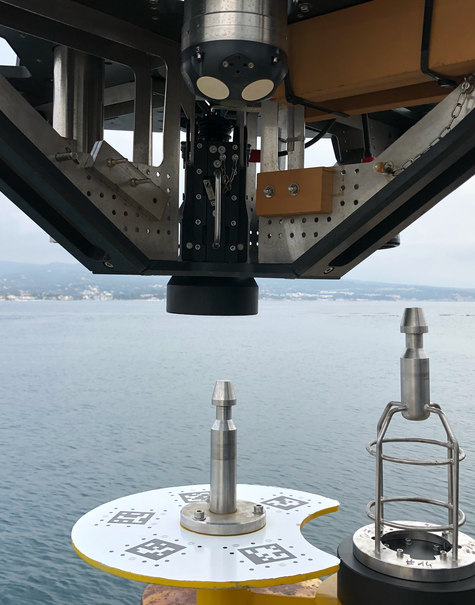
\includegraphics[width=0.99\textwidth]{imgs/latch_unlatched.png}
						\caption{Latch monté sur \atoll{} et crochet}
					\end{subfigure}
					\begin{subfigure}[b]{0.38\textwidth}
						\centering
						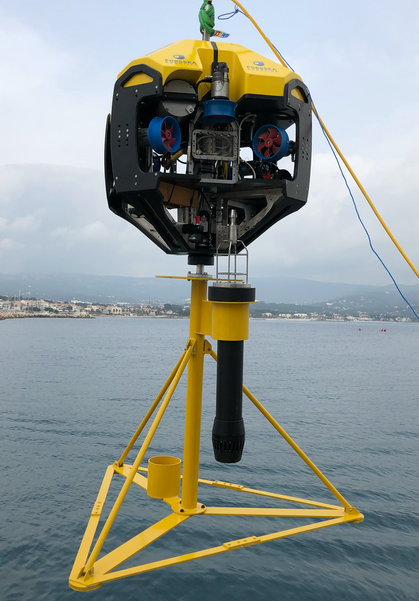
\includegraphics[width=\textwidth]{imgs/latch_latched.png}
						\caption{\atoll{} et structure sous-marine}
					\end{subfigure}
					\caption{Latch développé par \forssea{}}
					\label{fig:latch_photo}
				\end{figure}

				L'architecture logicielle du \textit{Latch} est présentée en \textsc{Figure}~\ref{fig:sa_latch}. Le composant reçoit deux informations de la part de l'implémentation logicielle : s'il est alimenté via le canal de communication \textit{power} et le signal de relâchement du crochet sur le canal \textit{release}. En retour, le crochet de levage renvoie son état à l'aide d'une sonde à effet Hall qui indique si le crochet est fermé ou ouvert sur le canal \textit{sensor}.

				\begin{figure}[!htb]
					\centering
					\includegraphics[width=0.8\textwidth]{build/diagrams/sa_latch.pdf}
					\caption{Architecture logicielle du \textit{Latch}}
					\label{fig:sa_latch}
				\end{figure}
							
				Le \plugin{} \gazebo{} développé afin de décrire le comportement du \textit{Latch} est basé sur la machine à états finis présentée en \textsc{Figure}~\ref{fig:latch_fsm}. L'idée est de créer une liaison encastrement dynamique entre le \textit{Latch} et la structure sous-marine à transporter. La logique implémentée dans la machine à états finis permet de simuler le fait que mécaniquement le crochet s'accroche automatiquement à un point d'attache de structure sous-marine qui rentrerait dans le composant, et que l'on ne commande que le relâchement de cette structure par l'ouverture du crochet.

				\begin{figure}[!htb]
					\centering
					\includegraphics[scale=0.8]{build/diagrams/latch_fsm.pdf}
					\caption{Machine à états du \textit{Latch}}
					\label{fig:latch_fsm}
				\end{figure}
		
			\subsubsection{SS309 Tilt}

				Le \textit{SS309 Tilt} est un composant commercialisé par l'entreprise \textit{Sidus Solutions} et qui permet dans les \gls{ROV}s d'orienter la caméra d'observation. Il est parfaitement étanche et comporte un jeu d'engrenages reliés à un moteur pas-à-pas pilotable en vitesse et en position. On demande ainsi au moteur de mettre l'axe à une certaine position et l'axe se déplace avec une vitesse de rotation spécifiée. La \textsc{Figure}~\ref{fig:ss309_tilt} présente le composant monté sur \argos{} avec la nacelle permettant de d'orienter la caméra d'observation.

				\begin{figure}[!htb]
					\centering
					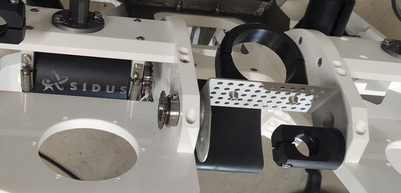
\includegraphics[width=0.6\textwidth]{imgs/ss309_tilt.png}
					\caption{SS309 tilt de \textit{Sidus Solutions} et nacelle pour \textit{Obscam}}
					\label{fig:ss309_tilt}
				\end{figure}
			
				Pour simuler cet aspect pilotable en vitesse de rotation et position, il faut passer par la simulation d'un moteur pas-à-pas. C'est un moteur composé de plusieurs bobinages créant ainsi plusieurs phases qui sont allumées successivement afin de réaliser une rotation de l'arbre moteur d'un certain incrément d'angle. Cet angle est défini par les caractéristiques du bobinage et n'est donc pas réglable. Ainsi, il est possible de connaître précisément la position du moteur en comptant le nombre d'incréments commandés, car l'arbre moteur ne peut prendre qu'un nombre fini d'angles et la vitesse avec laquelle le moteur se rend à cette position est commandée en allumant les phases à la vitesse désirée.

				L'architecture logicielle du \textit{SS309 Tilt} est présentée en \textsc{Figure}~\ref{fig:sa_tilt}. Le composant reçoit de la part de l'implémentation logicielle la position et la vitesse consigne sur les canaux \textit{command/position} et \textit{command/velocity}. Il est possible d'étendre le composant afin qu'il n'applique plus les consignes en envoyant un message sur le canal de communication \textit{power}. Enfin, il renvoie sa position et sa vitesse réelle récupérées dans l'environnement de simulation sur les canaux \textit{state/position} et \textit{state/velocity}.

				\begin{figure}[!htb]
					\centering
					\includegraphics[width=0.8\textwidth]{build/diagrams/sa_tilt.pdf}
					\caption{Architecture logicielle de la nacelle de caméra}
					\label{fig:sa_tilt}
				\end{figure}

				Nous allons à présent distinguer la position réelle de l'arbre moteur, la position cible et la position commandée. La position réelle est la position de l'arbre moteur dans le simulateur. La position cible est un multiple de l'incrément d'angle à laquelle doit se rendre le moteur à l'instant actuel. La position commandée est la position finale dans laquelle doit se retrouver l'arbre moteur et peut être une position réelle quelconque. Le moteur ne sera capable que de se rendre à la position multiple de la valeur de l'incrément d'angle la plus proche de la position commandée. La \textsc{Figure}~\ref{fig:tilt_position} reprends ces différentes notions. En commandant la vitesse à laquelle on incrémente la position cible, on contrôle l'axe en vitesse.

				\begin{figure}[!htb]
					\centering
					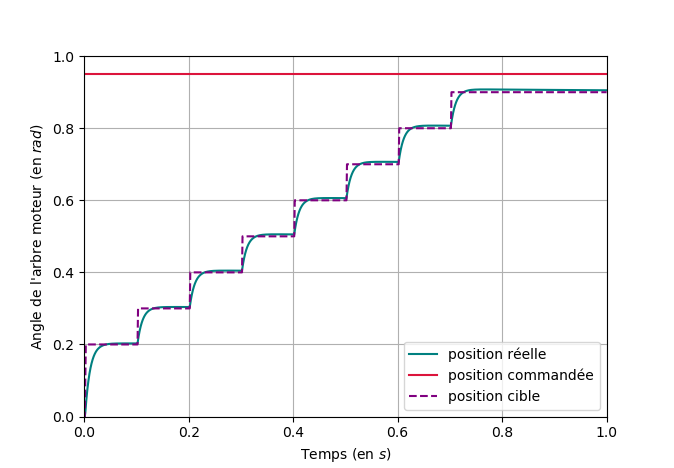
\includegraphics[width=0.6\textwidth]{imgs/stepper_motor.png}
					\caption{Simulation d'un moteur pas-à-pas}
					\label{fig:tilt_position}
				\end{figure}
				
				Pour ce qui est de l'implémentation de ce comportement dans \gazebo{}, on crée un \textit{Thread} qui va s'exécuter en boucle avec une vitesse variable. Cette vitesse sera fonction de la vitesse de commande du \textit{Tilt} notée $\omega_c$. A chaque tour de boucle, on incrémente donc la position cible de la valeur de l'incrément $d\theta$ si la différence entre la position réelle et la position commandée est plus grande que ce même incrément, et on attend le temps $h$ tel que $d\theta = h \omega_c$.

				\begin{algorithm}[!htb]
					\caption{Algorithme de simulation d'un moteur pas-à-pas}
					\label{algo:stepper_motor}
					\begin{algorithmic}
						\WHILE {true}
							\STATE read $\theta_r$, $\omega_c$
							\IF {$|\theta_c - \theta_r| > d\theta$}
								\STATE $\theta_t \leftarrow \theta_t + d\theta$
							\ENDIF
							\STATE $h \leftarrow \frac{d\theta}{\omega_c}$
							\STATE sleep $h$
						\ENDWHILE
					\end{algorithmic}
				\end{algorithm}

			\subsubsection{SPE75 Thrusters}
		
				Les \textit{SPE75 Thrusters} sont les propulseurs commercialisés par \textit{Sub-Atlantic} qui permettent aux robots de se déplacer et de s'orienter dans leur environnement. Ils sont composés d'un moteur permettant de mettre en mouvement des pâles qui vont générer une force dans la direction du propulseur. La \textsc{Figure}~\ref{fig:thrusters} représente trois propulseurs montés avec des orientations différentes sur \atoll{}, ce qui lui permet de se déplacer dans toutes les directions.

				\begin{figure}[!htb]
					\centering
					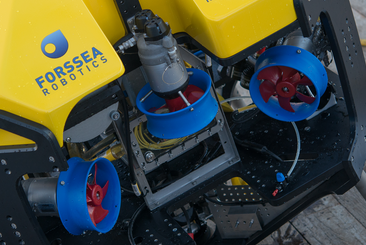
\includegraphics[width=0.5\textwidth]{imgs/spe75_thrusters.png}
					\caption{Trois propulseurs montés sur \atoll{}}
					\label{fig:thrusters}
				\end{figure}

				\begin{figure}[!htb]
					\centering
					\includegraphics[width=0.8\textwidth]{build/diagrams/sa_thruster.pdf}
					\caption{Architecture logicielle du propulseur}
					\label{fig:sa_thruster}
				\end{figure}
				
				L'\textit{Hardware Interface} propose une interface aux contrôleurs permettant d'appliquer une force suivant l'axe du propulseur au robot. Elle calcule ensuite la vitesse de rotation des pâles nécessaire à la création de cette force. \gazebo{} étant un simulateur dont la physique des solides est implémentée, le simple fait de faire tourner les pâles va générer des forces et des couples résistants sur le robot. Il ne reste donc qu'à appliquer les forces de poussée commandées qui ne sont pas implémentées dans le moteur physique.
				
				Le calcul de la vitesse de rotation des pâles en fonction de la force demandée est réalisé grâce à une interpolation de points de mesures faits sur un banc d'essai. L'idée est de faire tourner en eau le propulseur fixé sur un capteur de force à différentes vitesses constantes, et de mesurer les forces générées. Ensuite, en interpolant les points expérimentaux à l'aide de la librairie \textit{GSL}\footnote{\url{https://www.gnu.org/software/gsl/}} et de la fonctionnalité \textit{spline}, on peut calculer une vitesse de rotation à appliquer en fonction de la force demandée.
	
				Le \textit{Model Plugin} va se charger d'appliquer la force sur le propulseur et la vitesse de rotation aux pâles communiquée par l'\textit{Hardware Interface} à chaque pas de temps.

	\section{Simulation des robots}

		\subsection{Description du robot}

			Pour décrire les robots, il ne reste qu'à créer un fichier de description \textit{URDF} qui inclue autant de composants que nécessaires et les place correctement les uns par rapport aux autres.

		\subsection{Tests unitaires}
				
			Il est nécessaire de vérifier si tous les composants fonctionnent correctement et ont été convenablement ajoutés dans le robot. Pour cela il est courant d'implémenter des tests unitaires., qui vont permettre de tester unitairement les différentes fonctionnalités implémentées. Il est aussi nécessaire d'ajouter des tests liés aux choix de conception que nous avons fait, c’est-à-dire le fait d'avoir séparé les robots en composants simulés indépendamment les uns des autres.

			En effet, nous avons créé une description des \gls{ROV}s en incluant la description des sous-composants nécessaires. Il faut maintenant vérifier que la masse du robot, la position de son centre de gravité, sa matrice d'inertie, son volume et son centre de volume correspondent bien aux paramètres des robots. Pour ce faire, nous allons interpréter le fichier de description \textit{URDF} des robots en utilisant le module python \textit{urdfpy}\footnote{\url{https://github.com/mmatl/urdfpy}} afin de vérifier ces informations.

			\subsubsection{Vérification de la masse}

				Pour calculer la masse totale du robot, il suffit de sommer la masse de tous les composants. En considérant que le robot possède \textit{N} composants, et que $\forall i \in \llbracket 1; N \rrbracket, m_i$ représente la masse du \textit{i-ème} composant, et $m_{robot}$ la masse du robot, on a :

				\begin{equation}
					m_{robot} = \sum_{i=0}^{N}m_i
				\end{equation}

			\subsubsection{Vérification du centre de gravité}

				Pour calculer le centre de gravité du robot, on réalise une moyenne des centres de gravités pondérée par les masses des différents composants. En considérant que le robot possède \textit{N} composants, et que $\forall i \in \llbracket 1; N \rrbracket, m_i$ représente la masse du \textit{i-ème} composant et $G_i$ représente les coordonnées de son centre de gravité dans le repère monde, et $G_{robot}$ le centre de gravité du robot, on a :

				\begin{equation}
					G_{robot} = \frac{\sum_{i=0}^{N}m_i.G_i}{\sum_{i=0}^{N}m_i}
				\end{equation}

			\subsubsection{Vérification de la matrice d'inertie}

				Pour calculer la matrice d'inertie du robot, il faut sommer les inerties du robot. Définissons le repère $R_0$ associé au châssis du robot et le repère $R_i$ associé au composant \textit{i}. Partons de la matrice d'inertie disponible dans la description \textit{URDF} du robot exprimée dans le repère de chaque composant et en leur centre de gravité. Notons cette matrice $I_{i, R_i}(G_i)$. 
				
				Par cinématique directe, on peut obtenir la matrice de la transformation homogène $H_0^i$ entre les repères $R_0$ et $R_i$, qui exprime la rotation et la translation entre ces deux repères. Cette matrice est composée d'une matrice de rotation $R_{3, 3}$ et d'une matrice traduisant la translation $T_{3, 1}$ entre les deux solides.

				\begin{equation}
					H_{R_0}^{R_i} = \begin{bNiceArray}{CCC:C}[margin] &&& \\ & R_{3, 3} && T_{3, 1} \\ &&& \\ \hdottedline 0 & 0 & 0 & 1 \end{bNiceArray}
				\end{equation}

				En notant $I_{i, R_0}(G_i)$ la matrice d'inertie du i-ème composant exprimée en son centre de gravité dans le repère associé au châssis du robot, on peut exprimer le changement de base du tenseur d'inertie comme suit :

				\begin{equation}
					I_{i, R_0}(G_i) = R^T.I_{i, R_i}(G_i).R
				\end{equation}

				Puis, il faut exprimer le décalage entre l'origine du robot et le centre de gravité du composant. En utilisant la convention des coordonnées homogènes, et en notant $d^H = \begin{bmatrix}a & b & c & 1\end{bmatrix}^T$, on a :

				\begin{equation}
					d^H = H_0^i . G_i^H
				\end{equation}

				Ensuite on peut déplacer ce tenseur à l'origine du repère \textit{0} à l'aide de la formule de \textit{König-Huygens} :

				\begin{equation}
					I_{i, R_0}(O) = I_{i, R_0}(G_i) + m_i.\begin{bmatrix} b^2 + c^2 & -a.b & -a.c \\ -a.b & a^2 + c^2 & -b.c \\ -a.c & -b.c & a^2 + b^2 \end{bmatrix}
				\end{equation}

				Enfin, en possédant le tenseur d'inertie de chaque composant dans la base \textit{0} et au même point qui est l'origine du robot, on est en mesure de sommer ces inerties pour obtenir l'inertie totale du robot.

				\begin{equation}
					I_{robot, R_0}(O) = \sum_{i=0}^N I_{i, R_0}(O)
				\end{equation}

			\subsubsection{Vérification du volume}

				Pour calculer le volume total du robot, il suffit de sommer le volume de tous les composants. En considérant que le robot possède \textit{N} composants, et que $\forall i \in \llbracket 1; N \rrbracket, v_i$ représente le volume du \textit{i-ème} composant, et $v_{robot}$ le volume du robot, on a :

				\begin{equation}
					v_{robot} = \sum_{i=0}^{N}v_i
				\end{equation}

			\subsubsection{Vérification du centre de volume}

				Pour calculer le centre de volume du robot, on réalise une moyenne des centres de volume pondérée par le volume des différents composants. En considérant que le robot possède \textit{N} composants, et que $\forall i \in \llbracket 1; N \rrbracket, v_i$ représente le volume du \textit{i-ème} composant, $V_i$ représente les coordonnées du centre de volume dans le repère du robot, et $V_{robot}$ le volume du robot, on a :

				\begin{equation}
					V_{robot} = \frac{\sum_{i=0}^{N}v_i.V_i}{\sum_{i=0}^{N}v_i}
				\end{equation}


		\subsection{Tests unitaires d'\argos{}}

			Les différents tests unitaires ont été lancés sur les fichiers de descriptions \textit{URDF} d'\argos{} afin de vérifier que la composition du robot à base des différents composants définis ait bien les bonnes propriétés mécaniques. La \textsc{Table}~\ref{table:argos_unittest} présente les écarts entre le robot réel et la description réalisée à l'aide des composants. On y retrouve ainsi les résultats des tests unitaires pour \argos{}.
			
			\begin{table}[!htb]
				\centering
				\begin{adjustbox}{max width=\textwidth}
					\begin{tabular}{|c|c|c|c|c|}
						\hline
						\textbf{Grandeurs} & \textbf{Ecart avec la réalité} & \textbf{Marge d'erreur acceptée} & \textbf{Validation} \\
						\hline
						Masse (en $kg$) & $0.66$ & $\pm 1$ & \cmark \\
						\hline
						Position du Centre de Gravité (en $mm$) & $0.3 \quad 0.1 \quad 0.2$ & $\pm 1 \quad \pm 1 \quad \pm 1$ & \cmark \\
						\hline
						Matrice d'Inertie (en $m^2.kg$) & $\begin{bmatrix}0.2 & 0.03 & 0.11 \\ 0.03 & 0.23 & 0.08 \\ 0.11 & 0.08 & 0\end{bmatrix}$ & $\pm \begin{bmatrix}0.3 & 0.15 & 0.15 \\ 0.15 & 0.3 & 0.15 \\ 0.15 & 0.15 & 0.3\end{bmatrix}$ & \cmark \\
						\hline
						Volume (en $m^3$) & $0.002$ & $\pm 0.005$ & \cmark \\
						\hline
						Position du Centre de Volume (en $mm$) & $0.1 \quad 0.3 \quad -0.1$ & $\pm 5 \quad \pm 5 \quad \pm 5$ & \cmark \\
						\hline
					\end{tabular}
				\end{adjustbox}
				\caption{Tests unitaires d'\argos{}}
				\label{table:argos_unittest}
			\end{table}

			On voit que toutes les valeurs des écarts entre le robot réel et la description \textit{URDF} sont inférieures aux marges d'erreurs acceptables pour \argos{}, ce qui signifie que les tests unitaires sont bien validés pour ce robot.

		\subsection{Tests unitaires d'\atoll{}}

			\atoll{} étant encore en cours de conception mécanique, les différents composants n'ont pas encore leur position finale et certains composants évoluent encore comme le châssis de ce robot. C'est pourquoi la description \textit{URDF} d'\atoll{} n'est pas finie et donc les tests unitaires ne passent pas encore. On utilisera cependant le même principe pour tester la description de ce robot dès que sa conception sera figée.
			
	\section{Conclusion}
	
		En conclusion, nous avons divisé le travail de simulation des robots en simulant les composants uns à uns, afin de simplifier les développements et de mettre en commun un maximum de code entre les \gls{ROV}s. Pour la plupart des composants, un \plugin{} \gazebo{} a été nécessaire afin de décrire leur comportement dans l'environnement de simulation, et de pouvoir contrôler les robots avec le reste de l'implémentation logicielle. Enfin, nous nous sommes assurés que la simulation en composants donnait bien des paramètres mécaniques corrects pour les robots simulés par rapport au robot réel, afin d'avoir une simulation des robots ayant un comportement proche des \gls{ROV}s en conditions réelles.
